\documentclass[letterpaper,11pt]{article}
\usepackage[top=1.0in,bottom=1.0in,left=1.0in,right=1.0in]{geometry}
\usepackage{verbatim}
\usepackage{amssymb}
\usepackage{graphicx}
\usepackage{longtable}
\usepackage{amsfonts}
\usepackage{amsmath}
\usepackage{hyperref}
\usepackage{float}
\usepackage{setspace}

\usepackage{tikz}
\usetikzlibrary{positioning, arrows, decorations, shapes}
\usetikzlibrary{shapes.geometric,arrows}

\definecolor{illiniblue}{HTML}{B1C6E2}
\definecolor{illiniorange}{HTML}{f8c2a2}
\definecolor{pink}{HTML}{e2b1c2}
\definecolor{green}{HTML}{c2e2b1}
\definecolor{purple}{HTML}{b9b1e2}
\tikzstyle{snoblock} = [rectangle, 
text width=5em, text centered,  minimum height=0em]
\tikzstyle{noblock} = [rectangle, 
text width=5em, text centered,  minimum height=3em]
\tikzstyle{loblock} = [rectangle, draw, fill=illiniorange, 
text width=15em, text centered, rounded corners, minimum height=3em]
\tikzstyle{lbblock} = [rectangle, draw, fill=illiniblue, 
text width=15em, text centered, rounded corners, minimum height=3em]
\tikzstyle{oblock} = [rectangle, draw, fill=illiniorange, 
text width=10em, text centered, rounded corners, minimum height=3em]
\tikzstyle{bblock} = [rectangle, draw, fill=illiniblue, 
text width=10em, text centered, rounded corners, minimum height=3em]
\tikzstyle{arrow} = [thick,->,>=stealth]
\tikzstyle{pblock} = [rectangle, draw, fill=pink, 
text width=10em, text centered, rounded corners, minimum height=3em]
\tikzstyle{gblock} = [rectangle, draw, fill=green, 
text width=10em, text centered, rounded corners, minimum height=3em]
\tikzstyle{ppblock} = [rectangle, draw, fill=purple, 
text width=10em, text centered, rounded corners, minimum height=3em]
\tikzstyle{lppblock} = [rectangle, draw, fill=purple, 
text width=15em, text centered, rounded corners, minimum height=3em]
\tikzstyle{arrow} = [thick,->,>=stealth]
\tikzstyle{bbblock} = [rectangle, draw, fill=illiniblue, 
text width=1em, text centered, rounded corners, minimum height=1em]
\tikzstyle{boblock} = [rectangle, draw, fill=illiniorange, 
text width=1em, text centered, rounded corners, minimum height=1em]
\tikzstyle{bpblock} = [rectangle, draw, fill=pink, 
text width=1em, text centered, rounded corners, minimum height=1em]
\tikzstyle{bgblock} = [rectangle, draw, fill=green, 
text width=1em, text centered, rounded corners, minimum height=1em]
\tikzstyle{bppblock} = [rectangle, draw, fill=purple, 
text width=1em, text centered, rounded corners, minimum height=1em]

\author{Gwendolyn J. Chee}

\title{Generative Reactor Design}
\begin{document}
\maketitle
\hrulefill
\onehalfspacing

\section{Generative Design}
% What is generative design? How does it work? 
Generative design is an exploratory design method that autonomously 
generates optimal designs by iteratively varying design geometry 
to meet designer-defined performance metrics 
\cite{krish_practical_2011,oh_deep_2019}.
The human designer defines the design parameters and the generative 
design software helps the human designer create many solutions 
simultaneously \cite{autodesk_autodesk_2020}. 
This sometimes results in unanticipated unique solutions, that 
would have been difficult to discover using traditional methods
\cite{autodesk_autodesk_2020}.
Generative design varies the parameters of the problem definition
\cite{matejka_dream_2018}. 
At each iteration step, the design is evaluated on the 
performance metrics. 
Based on the results, the generative design algorithm changes the 
interval allowed for each design geometry variable, refining 
design constraints (problem definition) and moving towards 
designs that best meets performance metrics.

There is confusion to how generative design differs from other shape 
optimization tools. 
Generative design is more than topology optimization which has been 
around since 1988 \cite{bendsoe_generating_1988}. 
Topology optimization requires the user to start with a complete design 
and the software improves it by removing material, it answers the 
fundamental engineering question of how to place material in a domain space 
to obtain best structural performance \cite{sigmund_topology_2013}.   
Generative design does not require the user to start with a complete design, but 
instead a few design constraints. 
Table \ref{tab:compare} summarizes the differences between generative design and 
traditional design optimization tools. 

\begin{table}[h]
        \caption{Comparison of generative design and traditional design optimization tools
        \cite{autodesk_fusion_2020}.}
        \label{tab:compare}
        \centering
        \doublespacing
        \small
        \begin{tabular}{p{3.7cm}|p{5.5cm}p{6cm}}
        \hline
        \textbf{Point of Comparison} & \textbf{Generative Design} & \textbf{Traditional Design Optimization Tools}  \\ \hline
        Initial input & A few design constraints & Complete design \\ 
        No. of outcomes & Generates a wide set of designs that meets design constraints & Identifies one unique design that meets constraints \\   
        Solving strategies & Uses multiple strategies to solve design problem & Mainly uses topology optimization solutions \\ \hline
        \end{tabular}
\end{table}

% How does it actually work? What models? 

\subsection{State of Work}
Generative design is used in the following industries: 
automotive \cite{deplazes_autodesk_2019}, aerospace \cite{byrne_evolving_2014},
architecture, product design etc. 
For the automotive and aerospace industries, the goal of generative 
design is to decrease 
the weight of the vehicle while ensuring each part can continue to 
withstand the stresses and strains that are put on it within a 
safety factor. 
These industries can rely on commerical softwares such as 
Autodesk Fusion360 \cite{autodesk_autodesk_2020} and  
SolidWorks \cite{lombard_solidworks_2008}
to produce their generative designs, since these softwares have 
structural simulation-based generative design technology.  

\subsection{Genetic Algorithms}
Multi-objective design problems inevitably require a trade off between 
desirable attributes \cite{byrne_evolving_2014,simon_sciences_2019}. 
In nuclear reactor design there are many trade offs, one example is the 
trade-off between neutron economy and fuel enrichment. 
A reactor design must have sufficient neutron economy to ensure criticality, 
but must also have a low fuel enrichment to reduce proliferation risk.
Conflicting objectives means that there is no one perfect solution, but a set
of equally optimal solutions \cite{byrne_evolving_2014}.
Multi-objective problems are difficult to optimize, such problems 
cannot be handled by classical optimization methods such as gradient 
methods, because only the local optimum is found \cite{renner_genetic_2003}. 
Evolutionary algorithms have proven to be successful 
methods to optimize multi-objective problems \cite{krish_practical_2011} as 
they can find a solution near the global optimum \cite{renner_genetic_2003}. 
The most popular evolutionary algorithms used to solve multi-objective 
problems are genetic algorithms 
\cite{byrne_evolving_2014, krish_practical_2011}. 
Genetic algorithms imitate natural selection to evolve solutions 
by (1) maintaining a population of solutions, (2) allowing 
fitter solutions reproduce, and (3) letting lesser fit solutions die off, 
resulting in final solutions that are better than the previous generations 
\cite{renner_genetic_2003}. 
Figure \ref{fig:genetic_alg} depicts the iterative process of using a genetic 
algorithm to solve a problem. 
The key part of this process is defining evaluation and termination criteria. 

\begin{figure}[]
        \centering
        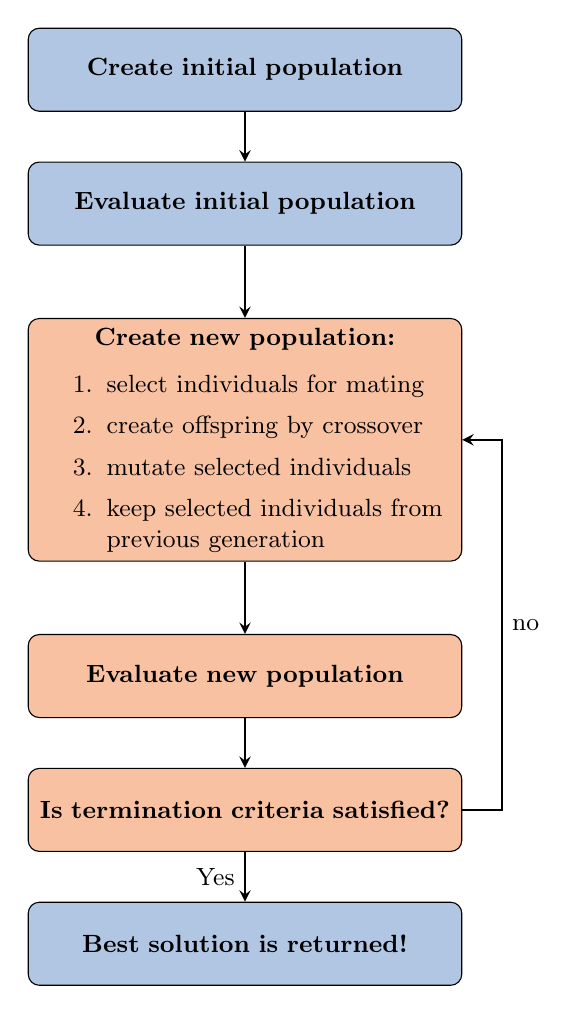
\begin{tikzpicture}[node distance=1.7cm]
                \tikzstyle{every node}=[font=\small]
                \node (1) [lbblock] {\textbf{Create initial population}};
                \node (2) [lbblock, below of=1] {\textbf{Evaluate initial population}};
                \node (3) [loblock, below of=2, yshift = -1.3cm] {\textbf{Create new population:} \\ 
                \begin{enumerate} \item select individuals for mating 
                                  \item create offspring by crossover 
                                  \item mutate selected individuals 
                                  \item keep selected individuals from previous generation
                                 \end{enumerate}};
                \node (4) [loblock, below of=3, yshift=-1.3cm] {\textbf{Evaluate new population}};
                \node (5) [loblock, below of=4] {\textbf{Is termination criteria satisfied?}};
                \node (6) [lbblock, below of=5] {\textbf{Best solution is returned!}};
                \draw [arrow] (1) -- (2);
                \draw [arrow] (2) -- (3);
                \draw [arrow] (3) -- (4);
                \draw [arrow] (4) -- (5);
                \draw [arrow] (5) -- node[anchor=east] {Yes} (6);
                \draw [arrow] (5) -- ([shift={(0.5cm,0cm)}]5.east)-- node[anchor=west] {no} ([shift={(0.5cm,0cm)}]3.east)--(3);
        \end{tikzpicture}
        \caption{Process of solving a problem with genetic algorithm 
        \cite{renner_genetic_2003}. Each iteration is a generation. }
        \label{fig:genetic_alg}
\end{figure}

Two types of genetic algorithms are typically used to solve shape 
optimization problems: parametric and cell. 
Parametric genetic algorithms optimize complex shapes by optimizing the shape 
of characteristics curves \cite{renner_genetic_2003}. 
Optimization of aerodynamic configurations \cite{makinen_multidisciplinary_1999}, 
and truss and bridge structures \cite{raich_evolving_2000} used parametric 
genetic algorithms.
Cell genetic algorithms represent the shape of an object to be optimized in 
small subdivided rectangular domains (pixels in 2D, voxels in 3D) 
\cite{renner_genetic_2003}. 
Figure \ref{fig:cell} shows an example of cell representation. 
Cell genetic algorithms are advantageous compared to parametric genetic 
algorithms since the initial structure and topology of the object need not 
be created and is instead developed through the iterative optimization 
process \cite{renner_genetic_2003}. 
Both parametric and cell genetic algorithms will be explored for the generative 
reactor design problem. 

\begin{figure}[]
	\begin{center}
		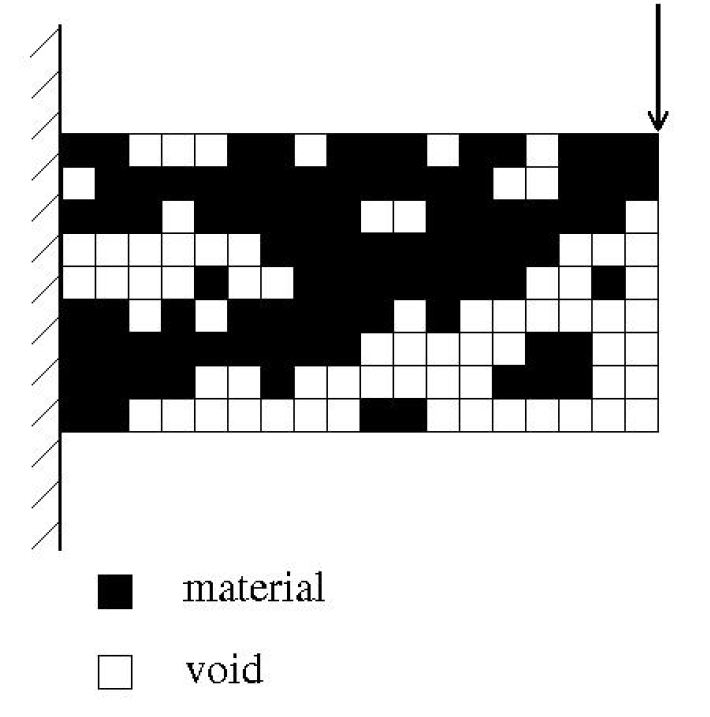
\includegraphics[scale=0.25]{./figures/cell.png}
        \end{center}	
        \caption{Cell representation in 2D \cite{renner_genetic_2003}.}
        \label{fig:cell}
\end{figure}

\section{Generative Reactor Design}
For nuclear reactors, generative design is constrained by 
variables such as mass or volume of fuel, fuel enrichment, effectiveness 
of heat transfer, effective neutron multiplication factor, etc. 
Nuclear reactors not only experience physical forces, they also
require evaluation of the neutronics, therefore generative design of 
a nuclear reactor cannot make use of tools such as Autodesk Fusion360. 
Therefore, a framework that couples well-developed advanced genetic algorithms 
with well-supported monte-carlo particle transport 
codes (Serpent \cite{leppanen_serpent_2014}, 
MCNP \cite{werner_mcnp6._2018}, etc.) and thermal hydraulics 
software (RELAP7 \cite{andrs_relap-7_2012} etc.)
must be created to successfully produce generative reactor designs. 

\subsection{Workflow}
% How the genetic algorithm is coupled with a CAD designer and analysis tool 
% (serpent/RELAP)
% CAD designer > grasshopper3d (see Bryne Paper)
Figure \ref{fig:workflow} depicts a framework for leveraging genetic algorithms
to design nuclear reactors. 
This is a general framework that does not specify algorithms or analytical 
softwares. 
Instead, it provides placeholders for algorithm and software types, so 
that a user may choose the types of algorithms and softwares they want to use in 
their mission towards using generative design to design a nuclear reactor. 
Table \ref{tab:examples} lists algorithm and software types that could be used 
in the framework. 

\begin{figure}[H]
        \centering
        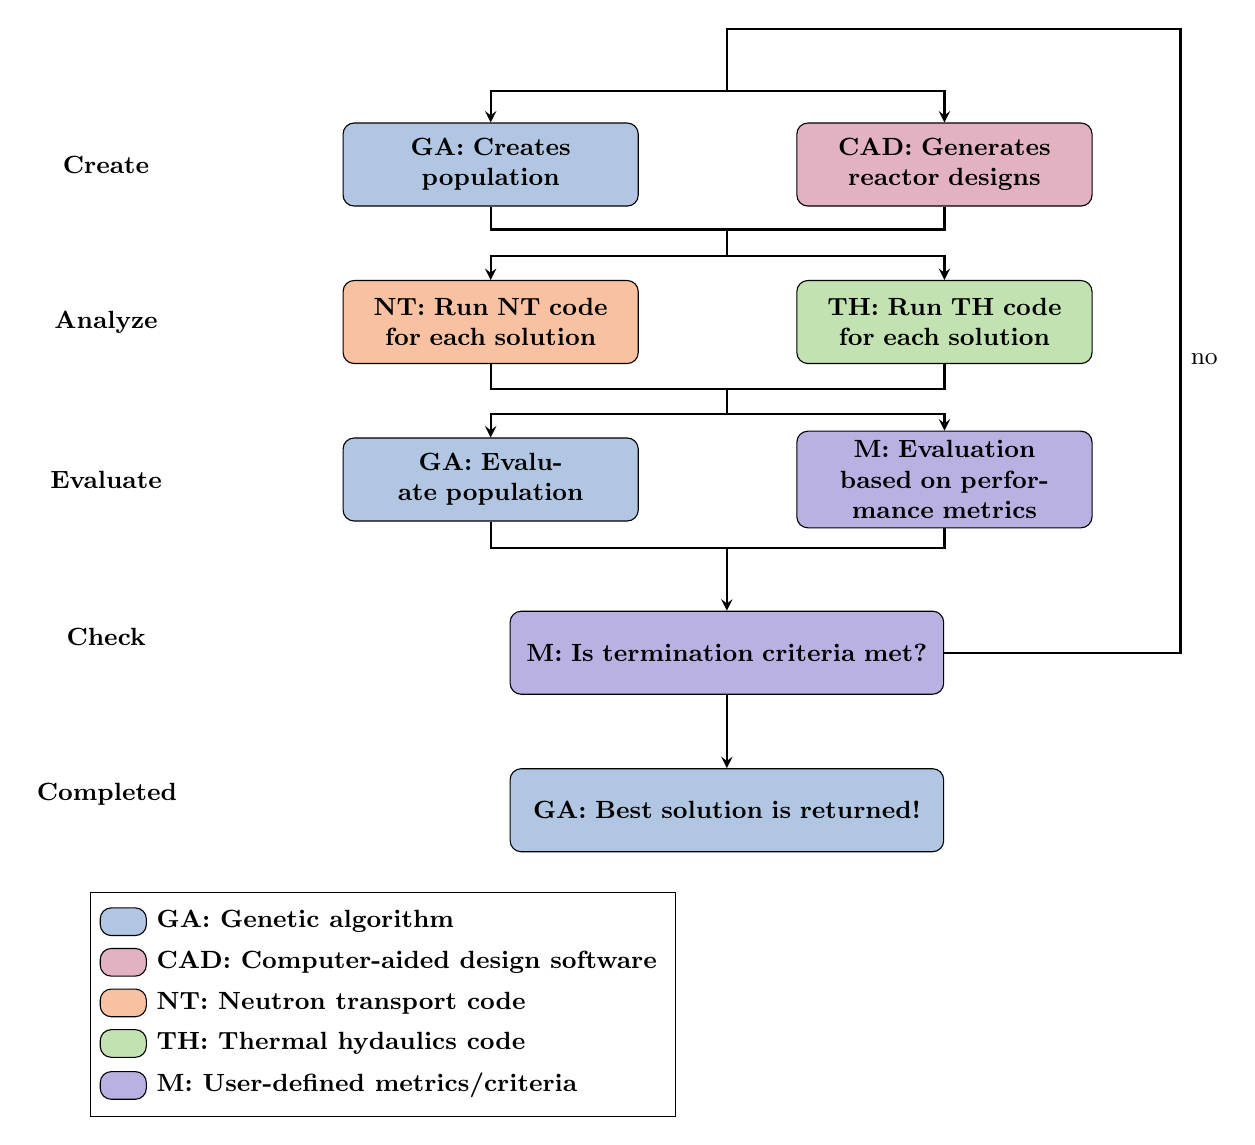
\begin{tikzpicture}[node distance=2cm]
                \tikzstyle{every node}=[font=\small]
                \node[anchor=west] (1) [noblock] {\textbf{Create}};
                \node (2) [bblock, right=of 1] {\textbf{GA: Creates population}};
                \node (3) [pblock, right=of 2] {\textbf{CAD: Generates reactor designs}};
                \node[anchor=west] (4) [noblock, below of= 1] {\textbf{Analyze}};
                \node (5) [oblock, below of =2]{\textbf{NT: Run NT code for each solution}};
                \node (6) [gblock, right=of 5]{\textbf{TH: Run TH code for each solution}};
                \node[anchor=west] (7) [noblock, below of= 4] {\textbf{Evaluate}};
                \node (8) [bblock, below of =5] {\textbf{GA: Evaluate population}};
                \node (9) [ppblock, right=of 8] {\textbf{M: Evaluation based on performance metrics}};
                \node[anchor=west] (10) [noblock, below of= 7] {\textbf{Check}};
                \node (11) [lppblock, below of=8, xshift=3cm, yshift=-0.2cm] {\textbf{M: Is termination criteria met?}};
                \node (16) [lbblock, below of = 11] {\textbf{GA: Best solution is returned!}};
                \node[anchor=west] (12) [snoblock, above of= 2, xshift=3cm, yshift=-1.1cm] {};
                \node[anchor=west] (13) [snoblock, below of=12,yshift=-0.15cm] {};
                \node[anchor=west] (14) [snoblock, below of=13,yshift=-0.02cm] {};
                \node[anchor=west] (15) [snoblock, below of=14,yshift=-0.02cm] {};
                \node[anchor=west] (17) [noblock, below of= 10] {\textbf{Completed}};
                \draw [-,thick] (11) -- ([shift={(3cm,0cm)}]11.east) |- node[anchor=west, yshift=-4.2cm] {no} ([shift={(0cm,0.7cm)}]12.north)--(12);
                \draw [arrow] (12) -- ([shift={(0cm,0cm)}]12.north) |- ([shift={(0cm,0.4cm)}]2.north)--(2);
                \draw [arrow] (12) -- ([shift={(0cm,0cm)}]12.north) |- ([shift={(0cm,0.4cm)}]3.north)--(3);
                \draw [-,thick] (2) -- ([shift={(0cm,0cm)}]2.south) |- ([shift={(0cm,0.3cm)}]13.north)--(13);
                \draw [-,thick] (3) -- ([shift={(0cm,0cm)}]3.south) |- ([shift={(0cm,0.3cm)}]13.north)--(13);
                \draw [arrow] (13) -- ([shift={(0cm,0cm)}]13.north) |- ([shift={(0cm,0.3cm)}]5.north)--(5);
                \draw [arrow] (13) -- ([shift={(0cm,0cm)}]13.north) |- ([shift={(0cm,0.3cm)}]6.north)--(6);
                \draw [-,thick] (5) -- ([shift={(0cm,0cm)}]5.south) |- ([shift={(0cm,0.3cm)}]14.north)--(14);
                \draw [-,thick] (6) -- ([shift={(0cm,0cm)}]6.south) |- ([shift={(0cm,0.3cm)}]14.north)--(14);
                \draw [arrow] (14) -- ([shift={(0cm,0cm)}]14.north) |- ([shift={(0cm,0.3cm)}]8.north)--(8);
                \draw [arrow] (14) -- ([shift={(0cm,0cm)}]14.north) |- ([shift={(0cm,0.21cm)}]9.north)--(9);
                \draw [-,thick] (8) -- ([shift={(0cm,0cm)}]8.south) |- ([shift={(0cm,0.3cm)}]15.north)--(15);
                \draw [-,thick] (9) -- ([shift={(0cm,0cm)}]9.south) |- ([shift={(0cm,0.3cm)}]15.north)--(15);
                \draw [arrow] (15) -- ([shift={(0cm,0cm)}]15.north) |- ([shift={(0cm,0.1cm)}]11.north)--(11);
                \draw [arrow] (11) -- ([shift={(0cm,0cm)}]11.south) |- ([shift={(0cm,0.1cm)}]16.north)--(16);
                \matrix [draw,below left,yshift=-0.5cm, xshift=-7cm] at (current bounding box.south east) {
                \node [bbblock,label=right:\textbf{GA: Genetic algorithm}] {}; \\
                \node [bpblock,label=right:\textbf{CAD: Computer-aided design software}] {}; \\
                \node [boblock,label=right:\textbf{NT: Neutron transport code}] {}; \\
                \node [bgblock,label=right:\textbf{TH: Thermal hydaulics code}] {}; \\
                \node [bppblock,label=right:\textbf{M: User-defined metrics/criteria}] {}; \\
                };
        \end{tikzpicture}
        \caption{Generative reactor design framework. Each component of the 
        framework is user-selected.}
        \label{fig:workflow}
\end{figure}

\begin{table}[h]
        \caption{Example algorithm and software types to populate generative reactor 
        design framework (Fig \ref{fig:workflow}).}
        \label{tab:examples}
        \centering
        \doublespacing
        \small
        \begin{tabular}{ll}
        \hline
        \textbf{Framework Component} & \textbf{Examples}\\ \hline
        Genetic algorithm & parametric, cell \cite{renner_genetic_2003} \\
        Computer-aided design software & Trelis \cite{noauthor_trelis_2018}, FreeCAD \cite{falck_freecad_2012}, SolidWorks \cite{lombard_solidworks_2008}, grasshopper3d \cite{rutten_grasshopper3d_2015} \\
        Neutron transport code & Serpent \cite{leppanen_serpent_2014}, MCNP \cite{werner_mcnp6._2018}, SCALE \cite{bucholz_scale:_1982}, OpenMC \cite{romano_openmc_2013} \\ 
        Thermal hydraulics code & RELAP5-3D \cite{strydom_comparison_2016}, RELAP7 \cite{andrs_relap-7_2012}, TRACE \cite{xu_multi-physics_2006}\\
        User-defined metrics/criteria & keff, heat transfer rate, fuel enrichment, mass of fuel \\ \hline
\end{tabular}
\end{table}


\bibliographystyle{plain}
\bibliography{2020-generative-reactor-design-lit-review}
\end{document}

